\chapter{Configuration and Testing}
\label{configurationandtesting}
This chapter will contain the configuration of all nodes of the concept. In addition the newly developed nodes have to be tested as well as the entire navigation concept.


The structure of this chapter is to address the outer nodes of the navigation concept first and then move to the inner nodes.\\


\section{URDF and Robot State Publisher}

\section{Gazebo}

\subsection{Plugins}

\section{Filter}

\subsection{road\_detection}

\subsection{laser\_filter}

\subsection{robot\_localization}

When looking at the odometry published by the differntial drive plugin in Figiure \ref{} we notice, that it has rotational error.\\

\begin{figure}
	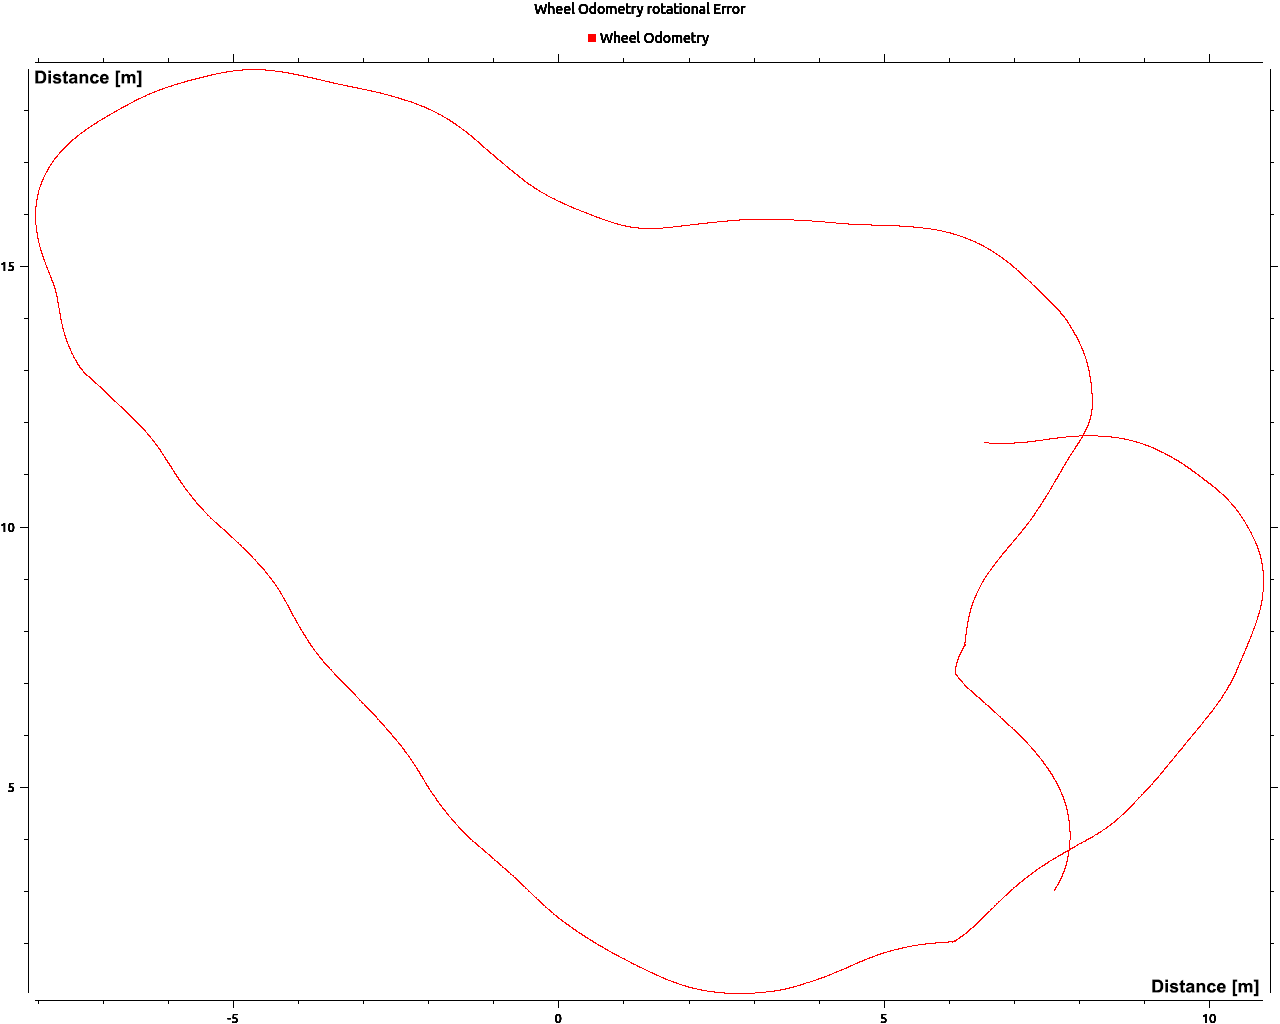
\includegraphics[width=\textwidth]{Pictures/rot error}
	\caption{Odometry from wheel encoder}
	\label{wheel odom}

\end{figure}


The following nodes require odometry:
\begin{itemize}
	\item cartographer
	\item move\_base
	\item posefinder
\end{itemize}

To improve the odometry the ROS package robot\_localization can be used. It provides an extended kalman filter for the fusion of sensor data for odometry.\\

To counter the rotational error the IMU and the encoder-odometry will be fused.\\

The IMU provides the following data:
\begin{itemize}
	\item orientation
	\item angular velocity
	\item linear acceleration
\end{itemize}

Based on the knowledge about the usecase of the IMU it does not make a lot of sense to fuse all of the data of the IMU and the kalman filter needs to be configured accordingly.\\


At first the measurements for three dimensional use can be removed, which are:
\begin{itemize}
	\item pitch angle and velocity
	\item roll angle and velocity
	\item linear acceleration in z
\end{itemize}

The IMU is used for localization purposes, therefore the linear acceleration data are not interesting, since they would need to be integrated twice to be used for the pose. This would amplify every little error in acceleration over time making the odometry unreliable over time.\\

Accordingly the only things fused from the imu are the yaw orientation and velocity.\\

Just like the IMU data the integration of the wheel-odometry data has to be discussed which consist only from linear and angular velocity.\\
Here the most interesting part is the y velocity since the robot is relying on differential drive steering and therefore not able to have y accelerations other than drift.\\

In contrast to the acceleration values of the IMU the y velocity will be included since according to Tom Moore \cite{robot\_localizationconfiguration} it will give certainty that the robot has not moved in the y direction. Obviously the x and yaw velocity has to be included aswell.
The position component of the wheel-odometry on the other hand will not be used, based on the fact that the position is already derived from the velocitys this would include the same data twice.\\

Unfortunately this does not solve the problem of the odometry correction yet. As visible in Figure \ref{pose comparison wheel odom + IMU} the odometry of the extended kalman filter has large jumps in it compared to the wheel-odometry. When observing it in real time the ekf odometry starts to drift and jumps back after a certain amount of time.\\
Looking at the linear velocities of both the ekf and the wheel odometry in Figure \ref{} it is noticeable that the ekf filter does estimate a continuous acceleration, whereas the velocity of the wheel encoders actually decreases.\\



\begin{figure}
	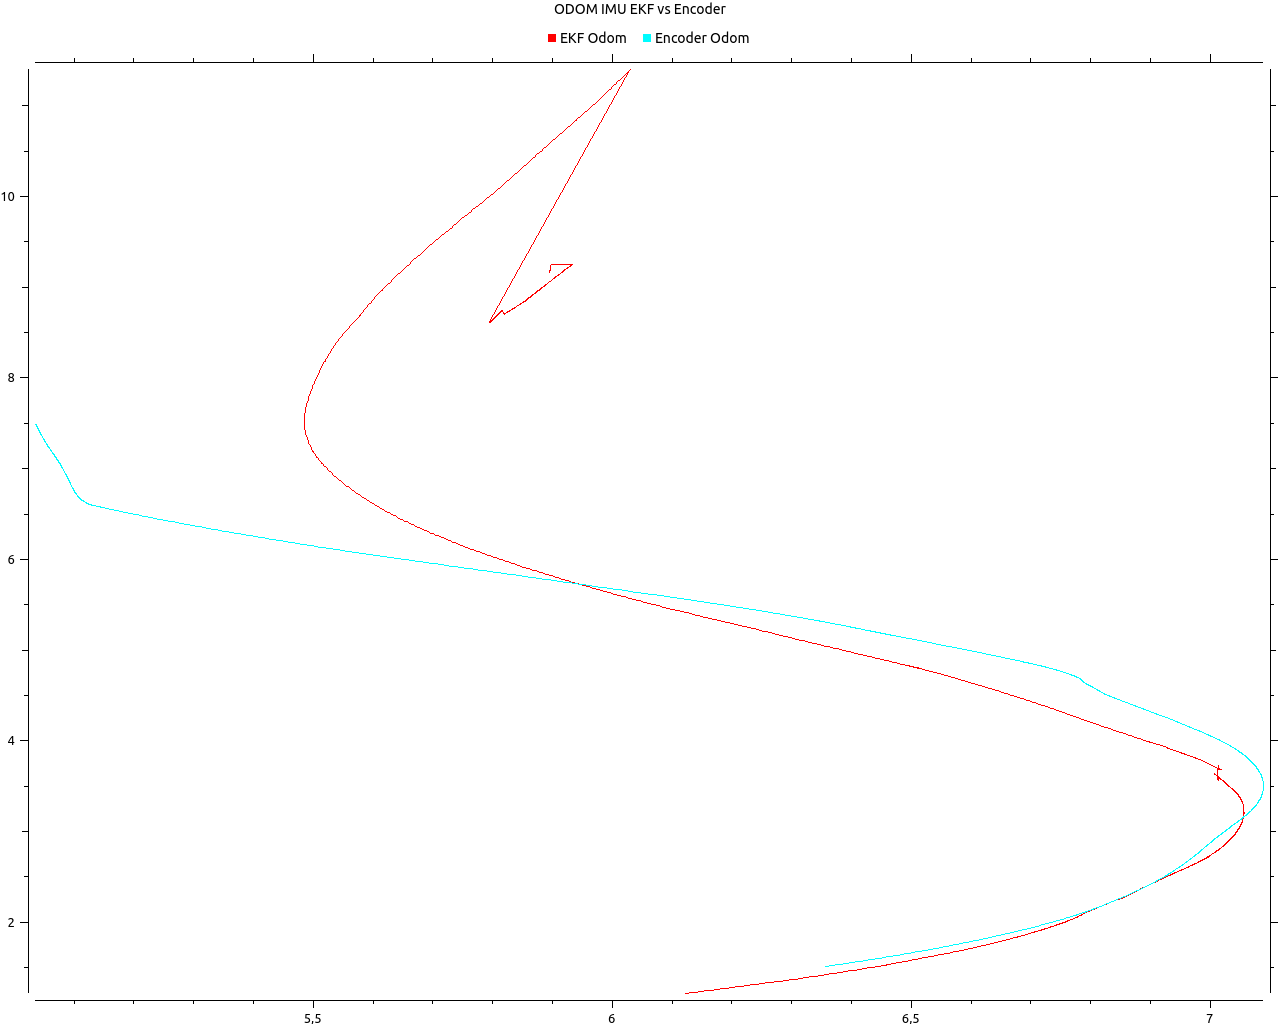
\includegraphics[width=\textwidth]{Pictures/odom pose comp}
	\caption{pose comparison wheel odom + IMU}
	\label{pose comparison wheel odom + IMU}

\end{figure}

\begin{figure}
	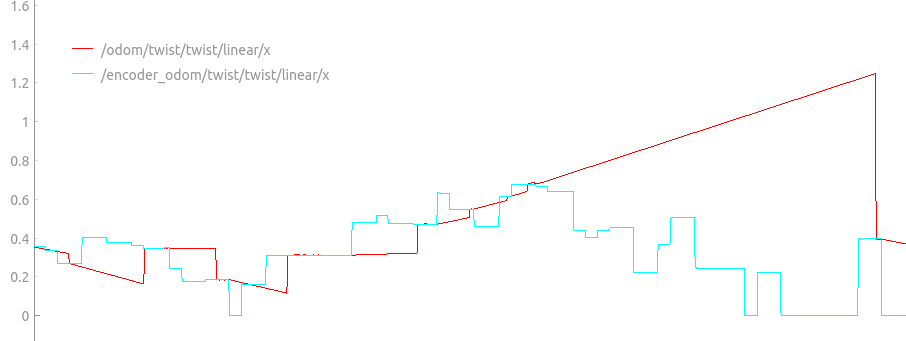
\includegraphics[width=\textwidth]{Pictures/comparison odom}
	\caption{velocity comparison wheel odom + IMU}
	\label{velocity comparison wheel odom + IMU}

\end{figure}


To fix this a logical approach is to include more data about the robots movement. Fortunately robot\_localization has an input for command velocities such as velocities produced by move base.\\
It is very important to set the control timeout to a value that is larger than the cycle time of move\_base. Otherwise this will lead to translational offsets caused by too low estimate for the velocities like shown in Figure \ref{velwithcmd}.

\begin{figure}
	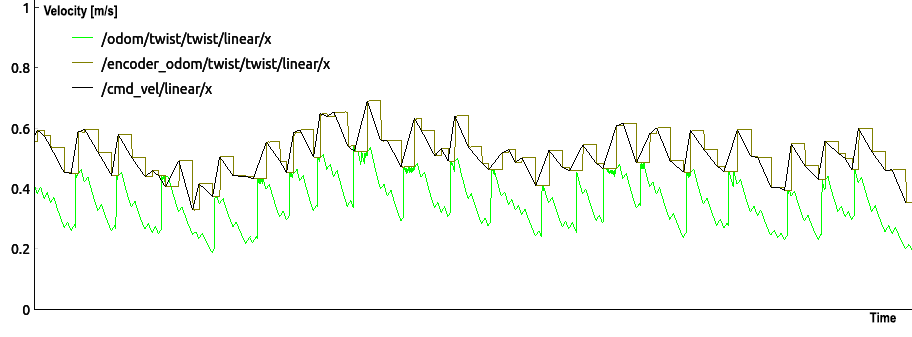
\includegraphics[width=\textwidth]{Pictures/velocity comp}
	\caption{velocity offset caused by too low control timout}
	\label{velocity offset}

\end{figure}


After the inclusion of the command velocity the acceleration limits can be set equal to the limits in the local planner.

When observing both the pose and velocities again it is noticeable, that the odometry has drastically improved as pictured in Figure \ref{Odometry comparison wheel odomIMUcmdvel}, equally the velocities stay closer together as pictured in \ref{velocity comparison wheel odomIMUcmdvel}.

\begin{figure}
	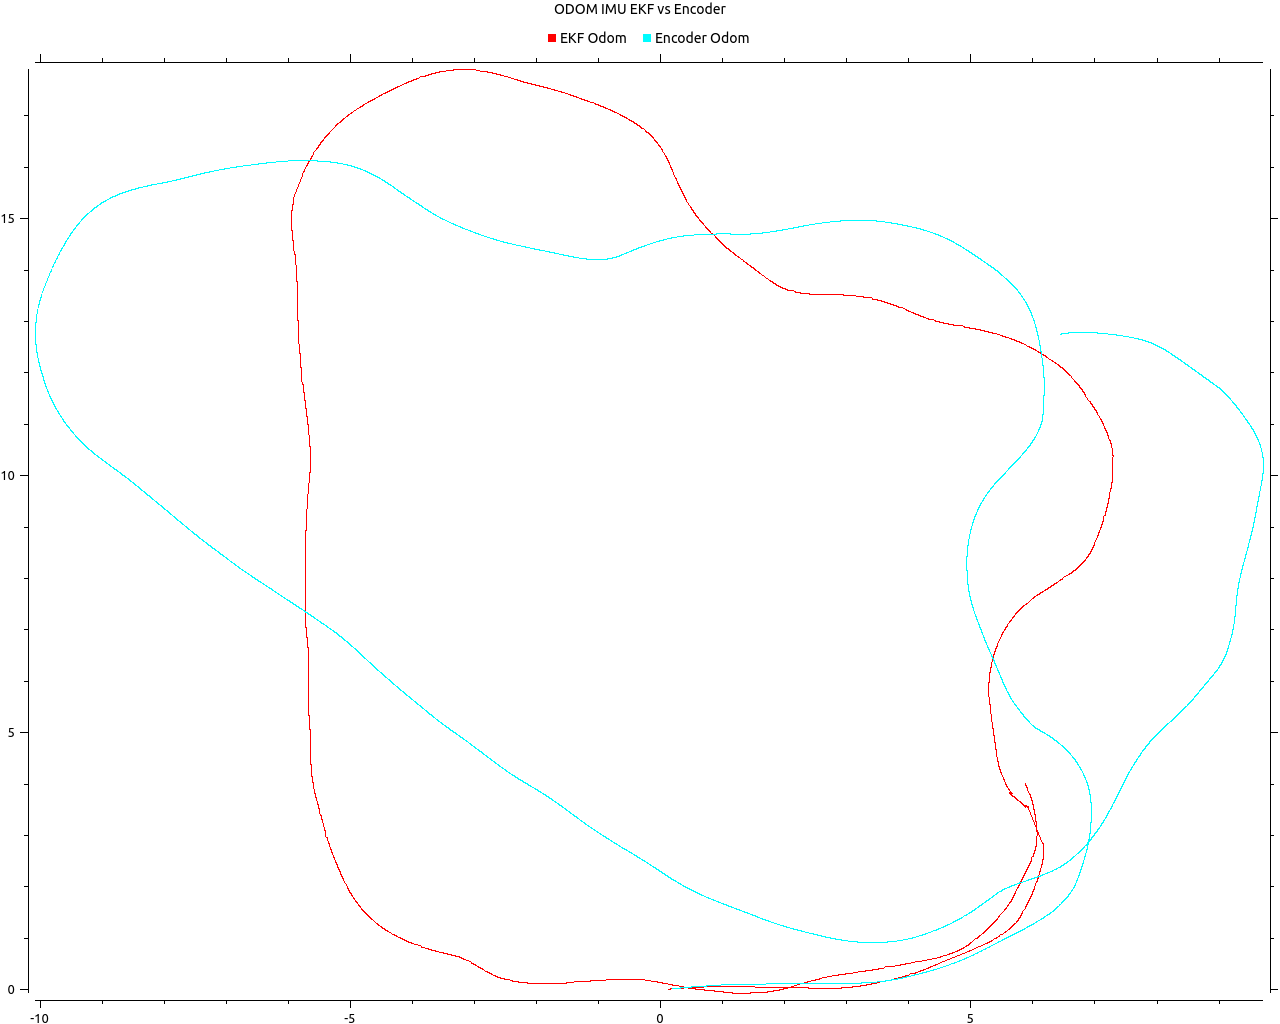
\includegraphics[width=\textwidth]{Pictures/odom after one round}
	\caption{Odometry comparison wheel odom + IMU + cmd\_vel}
	\label{Odometry comparison wheel odomIMUcmdvel}

\end{figure}
\begin{figure}
	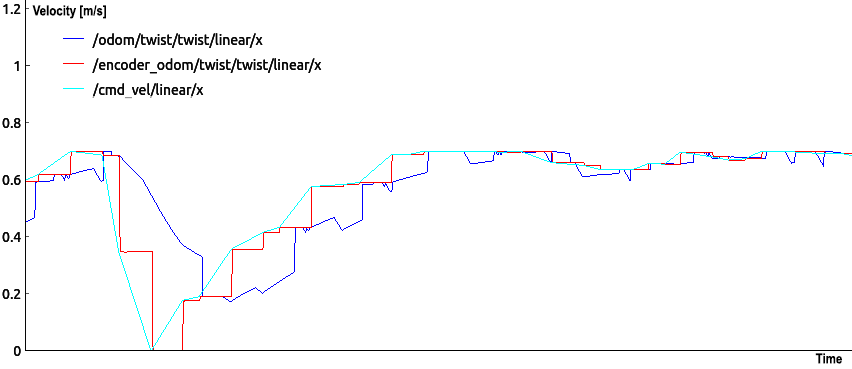
\includegraphics[width=\textwidth]{Pictures/circle vel}
	\caption{Velocity comparison with cmd\_vel}
	\label{velwithcmd}
\end{figure}



\begin{figure}
	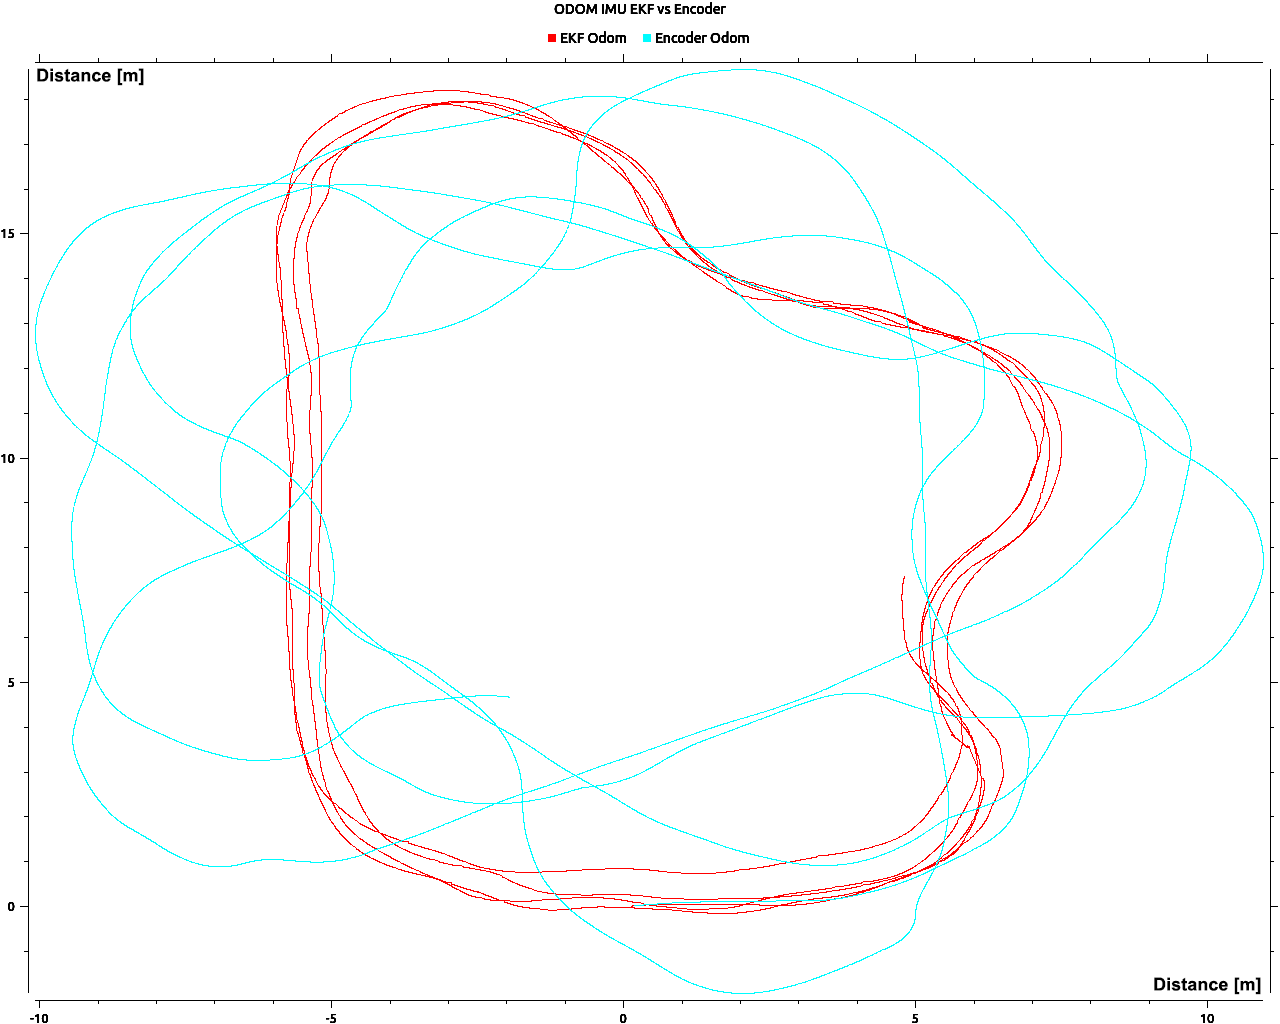
\includegraphics[width=\textwidth]{Pictures/odom comp multiple rounds}
	\caption{Odom comparison multiple rounds}
	\label{Odom comparison multiple rounds}

\end{figure}

Even after four rounds the odometry has not gained a large error in both translational and rotational as pictured in Figure \ref{Odom comparison multiple rounds}, furthermore the difference between the original odometry of the wheel encoders to the odometry from robot localization is quite remarkable.

Finally after the rotantional and translational errors are marginal the scale of the odometry needs to be checked.
To isolate the different errors from the scaling error a circular track is build with a radius of 10 meter. Since the turning radius is constant this isolates the rotational error which can be seen at the graph of the wheel odometry in Figure \ref{circular track}.\\
The radius has to be chosen that high to display the potential error better.\\

Since the robot is driving on the lane and not on the middle road marking the expected radius is 10,45 meter. When evaluating the EKF odom in Figure \ref{circular track} we see that the scale is very precise.
 
\begin{figure}
	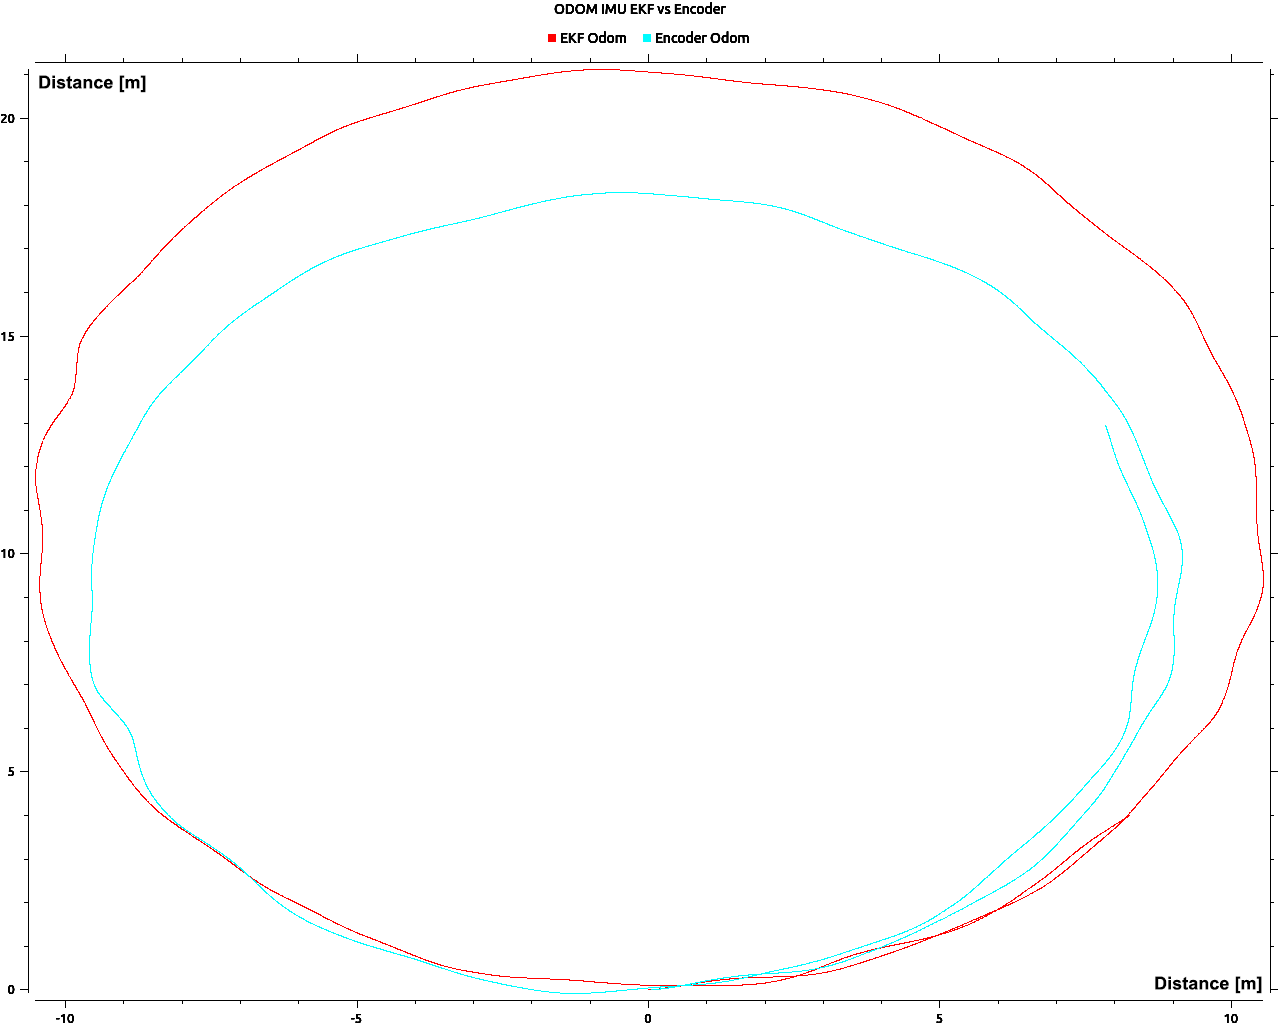
\includegraphics[width=\textwidth]{Pictures/circle odom}
	\caption{Odom comparison circular track}
	\label{circular track}

\end{figure}
 
\subsection{markfreespace}


\section{Cartographer}
The goal of this node is to produce a map that gets more reliable over time.\\

Unfortunately the data available for Cartographer is very self simillar, meaning a straight road will allways look the same and therefore does not have sufficient features for proper loop closure. In contrast to the points from the road detection the lidar can actually supply such features and will therefore be a good improvement for the resulting map.\\

But it is not guaranteed that the lidar will even sees anything the SLAM algorithm has to work with the points of the road detection only aswell.

The basic configuration of cartographer is purely based on the setup of the robot. In this case cartographer is supposed to use lidar and the points of the road detection at the same time. To reduce the amount of times one of the sensor doesn't see anything these will need to be merged in the markfreespace node and cartographer will receive one PointCloud2 only.\\
To improve the map further the odometry supplied by the robot\_localization package is used as an input, aswell as the IMU.

Furthermore cartographer will be set to 2d map building.


\subsection{Tuning}
With the basic configuration cartographer is not able to provide a reliable map and a tuning procedure has to be performed. Here the general recommendation of the tuning guide should be followed, which states to tune local SLAM first and disabling global slam while doing so \cite{cartographertuning}.
To tune the local SLAM the parameter of the tracjectory builder have to be adjusted.\\
The trajectory builder contains a scan-matcher, which will compare incoming sensor data a tries to align it with each other as good as possible. This behavior can be tuned by configuring the size of the linear and angular search windows and the weight for the rotation and translation of the incoming scans.\\
One more important setting is the size of the sub maps. These can be adjusted by the amount of scans they contain. Since the submaps will consist out of the scan matched obstacles it is important to set the size of the submaps not to high, if the incoming data will be very self simillar. Otherwise the scanmatcher will combine too many scans while shifting them over each other since they look so simillar. This results in both rotational and translational error.\\
As soon as the local SLAM produces a reliable result after multiple rounds of the robot the global SLAM can be activated and tuned.\\

The global SLAM has two options of combining the submaps the loop-closure, which will check, if the robot was at this spot already, and a scanmatcher, which will try to match the submaps to the current scan. For both of these the weights can be adjusted individually and like in the local SLAM the size of the window for translation and rotation can be adjusted. Reducing the window size to a minimum is aswell important when dealing with self simillar data, so the submaps will not be shifted on top of each other. The size should be chosen so the global SLAM can still correct errors of the individual submaps 
With these values and the submaps the global planner calculates constraints between the maps which will be valued between 0 and 1. These constraints can be blocked with a threshold value that will block constraints with a smaller value. like this the computation time can be drastically reduced and only the important constraints will be processed. Furthermore the weighting of the Pose of the odometry and the local SLAM can be adjusted, which can be usefull with bad odometry.

\subsection{Testing}
Testing of the SLAM will mostly consist out of a Black-Box Test meaning the only things that will be observed is the output and therefore the map.
The SLAM will be tested in the following cases:
\begin{itemize}
	\item Data purely from the road detection.
	\item Data from road detection and lidar scan with obstacles on the side of the road.
	\item Data from road detection and lidar scan with obstacles on the road.
	\item Long duration test with both road detection and lidar scan with obstacles on the side of the road.
\end{itemize}

During all of these test the navigation will solely work with the predicted goals since it is yet unsure if the SLAM map is even usable. Furthermore the same tuning will be used for all tests.\\

\textbf{Data purely from localization:}\\
The reason for this test is to check if the SLAM algorithm can handle Mapping with as least information as possible. This will make loop-closure difficult and cartographer has to work with the self simillar data only.\\
The aim is, that the robot can drive multiple rounds, on the track and cartographer produces an optimized map with little unmatched submaps and well connected road markings.\\
As long as the localization in the map works nicely the distortion in the map is less important and will not be tested.\\

The following pictures contain the SLAM map after the \nth{1},\nth{3} and \nth{5} round.\\

\todo{include pictures of test}

\textbf{Data purely from localization and lidar scan with obstacles on the side of the road:}\\

\textbf{Data purely from localization and lidar scan with obstacles on the road:}\\
This test is meant to be the worst case for the SLAM algorithm during navigation. The purpose is to check how cartographer handles data loss during obstacle avoidance and lane swapping.
The obstacles will be placed in two corners and therefore in the edge case where the camera has the worst chance of seeing the road because of the steering angle, aswell as on the straight section of the road to cover the case where the camera can not see the road during merging on an other lane. Furthermore the obstacles will be placed far enough apart so the lidar has only vision on one at the same time.\\

\textbf{Long duration test with both road detection and lidar scan with obstacles on the side of the road:}\\
Cartographer seems to not merge old submaps but process all of them allways, which will progressively increase computational load. Since the SLAM is supposed to be used during mapping this can become important with a lot of sensor inputs that offer constraint potential (lidar data) and long runtime.
The same setup as in the \nth{2} test will be used but the focus is on the moment, at which cartographer cannot optimize in real time caused by too many submaps and constraints.\\


\textbf{Discussion of the test results}\\
As proven by the first two tests, cartographer is well tuned and the map would be useable for goal extraction. The submaps are well alligned and the map has no huge translational or rotational offset.\\
The \nth{3} and \nth{4} test on the other hand display the limitations of the slam algorithm.\\
When obstacles are located on the right lane the allignment of the submaps fails and a lot of submaps cant be attached to the rest of the map. After passing the obstacle the map gets better again, which would imply that the map could be good enough for goal extraction, if no obstacle is near the robot.\\
The \nth{4} test proves that cartographer is not usable in SLAM mode during long time navigation an a circuit. This is caused that too many submaps are close to each other that share features for a constraint.

Based on these test results it is not feasible to use the SLAM map for navigation with obstacles on the road, since the map is just not reliable enough and it is not certain of there are obstacles on the road or not. 
\section{PoseFinder}


\section{Costmaps}
Based on the fact that both planners are responsible for different tasks the configuration of the individual costmaps need to fulfill different tasks too. The requirements of the two planners will be compared in order to determine the configuration of their individual costmap.\\

As described in the theoretical knowledge of this thesis the costmap are structured in layers. This means that the data can be evaluated by different plugins before it will be combined into the real costmap.\\

It makes sense to first take a look at the general behaviour, that both planners share. In this case it is obstacle avoidance. This means that the lethal obstacles need to be marked in both costmaps.\\

To implement this the provided plugin obstacle\_layer can be used. It will take incoming sensor data (sensor\_msgs::PointCloud or sensor\_msgs::LaserScan) and mark the points in the costmap.\\

Since the data here comes form the road detection and a lidar and both have a certain resolution it is unsure, if the result of a scanned obstacle in the costmap is actually a closed line or just points, since this highly relies on the resolution of the sensors and the costmap.\\

To fill theses gaps in the costmap the provided plugin inflation\_layer can be used. It will inflate only the lethal obstacles in the costmap with a configurable cost distribution.\\

This setup is already enough for the local costmap, where as the global planner needs to fulfill the quest of changing lanes if necessary but all-ways preferring the right lane. For this a custom plugin will be needed that makes the transition to the left lane more expensive but still possible.


The final layer plugin setup of the costmaps results in the following:

\textbf{global costmap}
\begin{itemize}
	\item obstacle layer
	\item inflation layer
	\item dynamic cost layer
\end{itemize}

\textbf{local costmap}
\begin{itemize}
	\item obstacle layer
	\item inflation layer
\end{itemize}

The costmaps will both have the same size that should allways be larger than the distance, at which the goalfinder searches for goals.

Since both costmaps are rolling window costmaps they will reference the continuos frame ``odom'' and move with the frame ``base\_footprint''.

Counterintuitively the robot radius needs to be set smaller than the robot actually is. Otherwise the slightly moving obstacles collide with the footprint and the global planner can not produce a valid path that the local planner can follow.\\
This footprint is only considered by the global planner, which is only required to provide a rough path. The local planner has its own setting for a footprint, therefore the obstacle avoidance will still work as expected.

The last remaining settings are the resolutions and the frequencies of the costmaps, which are chosen based on the performance of the navigation and the computational load.


\subsection{dynamic\_cost\_layer}
Enhancing to the plugins provided in the navigation stack this layer handles inflation of cells with a configurable cost decay and radius. While this seems to be similar to the provided inflation layer, this offers way more flexibility since it will inflate specific points by their individual radius and cost distribution and not just every lethal one by one fixed distribution.\\

This behavior can be used to inflate the left road marking in the global costmap to force the global plan on the right side of the road. The plugin can also be used to inflate cells with zero cost, which is useful to guarantee a cost free right lane or to give some free space around obstacles located on the road.\\

The layer receives a message of type sensor\_msgs::PointCloud on a configurable topic. This PointCloud is expected to feature Channel Values for the inflation radius, the maximal and the minimal cost for each individual point.\\

Since we can't assume that the incoming points will be in the frame of the costmap the points in the costmap have to be transformed into the right frame using tf2.\\

To minimize the computation load a bresenham based algorithm for the circle rasterization will be used.\cite{ComputerGraphics} Now the point symmetry around the cell can be used to further minimize the computational load and only $\frac{1}{8}$th of the circle has to be computed. The rasterization process can be described by the following image.\\

\begin{figure}[H]
	\centering
	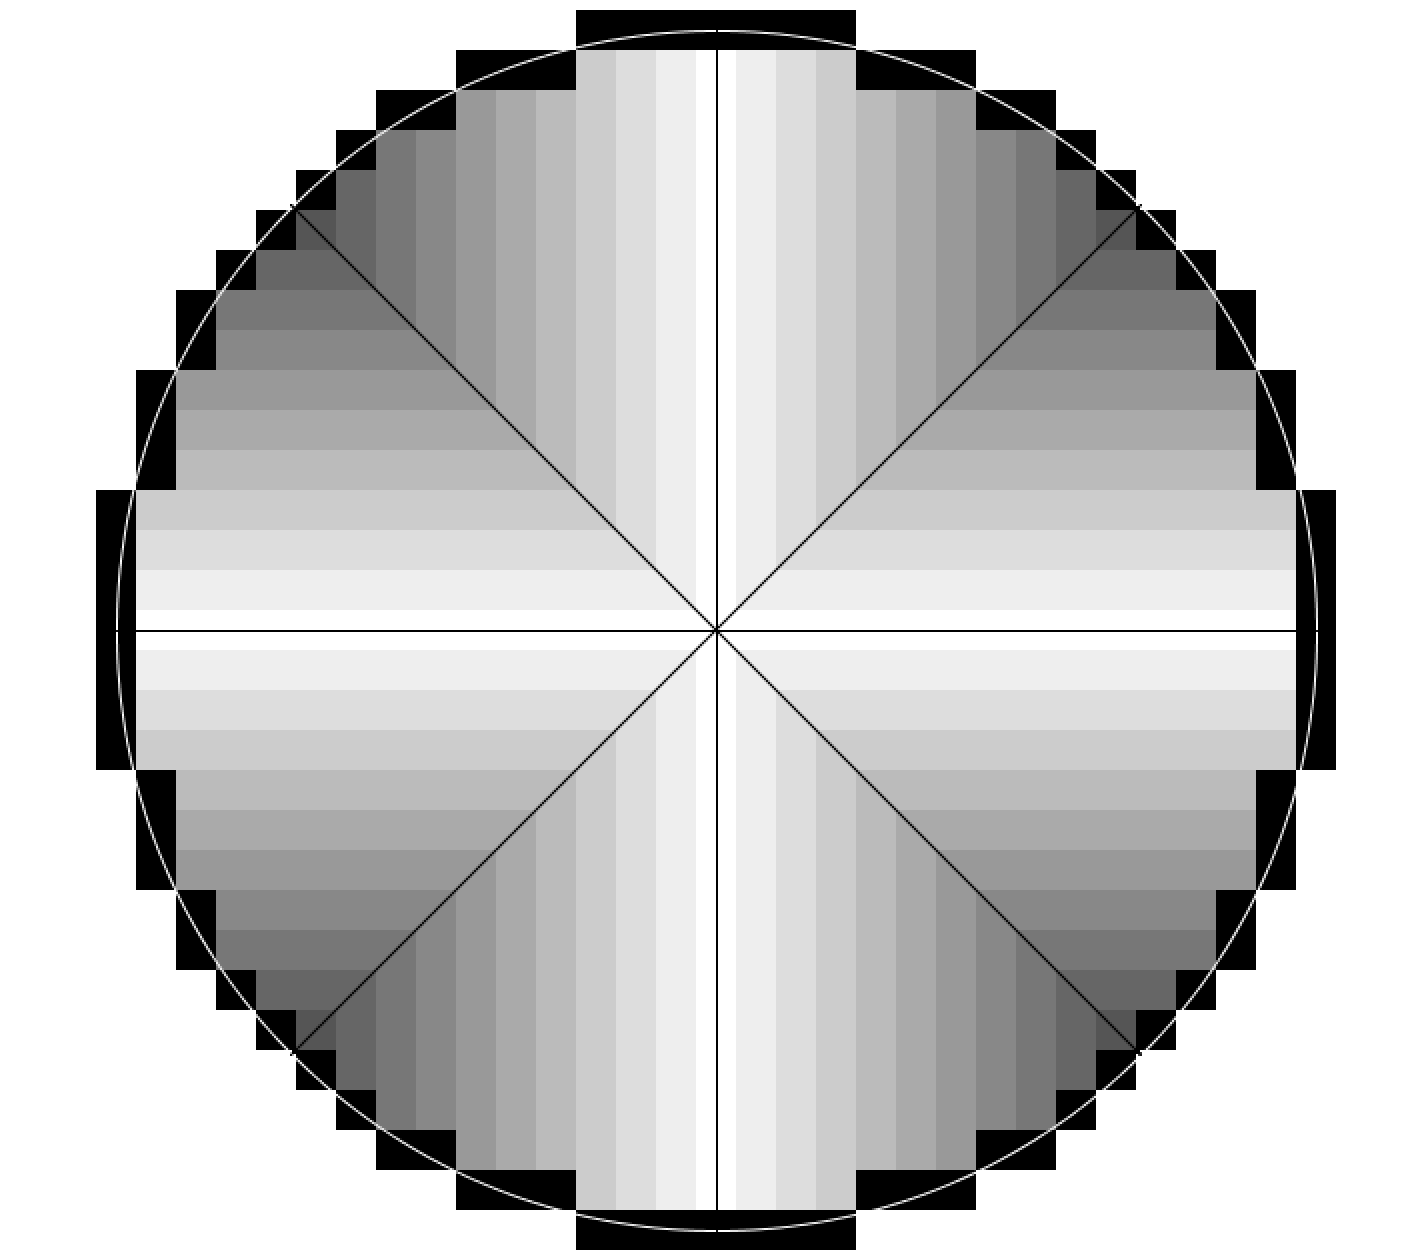
\includegraphics[width=.5\textwidth]{Pictures/rasterization}
	\caption{modified bresenham rasterization with efficient surface filling}
	\label{rasterization}
\end{figure}


Adding to the typical behavior of the bresenham rasterization the area of the circle will be filled using the point symmetry and by skipping overlapping points of the lines like in Figure \ref{rasterization}. Here it is visible, that every row with the same color is only calculated once and then projected in all eight octants. The Black cells on the perimeter are the rasterized cells of the bresenham algorithm.

The cells within the circles perimeter are filled with the cost specified for that point. For this the following linear decaying \nth{1} degree function will be used which requires the computation of the distance of the rasterized cell to the center of the circle.

\[cost(distance)=maxcost-distance*\frac{maxcost-mincost}{radius}\]\\
with: \[distance=\sqrt{cell.x^2+cell.y^2}\]

 Since this will still require the usage of a square root for each cell in the circle This will be optimized as well.\\

The goal here is to use a function that contains only the squared distance, which still represents a decaying trend. This requirement rules out every function with an odd degree, as well as all functions with an x offset. This leaves all functions with an even degree from which we choose the \nth{2} degree function to reduce square operators. The comparison between the two functions can be seen in the picture below.

\[cost(distance)=maxcost-distance^2*\frac{maxcost-mincost}{radius^2}\]\\

\begin{figure}[H]
	\begin{center}
	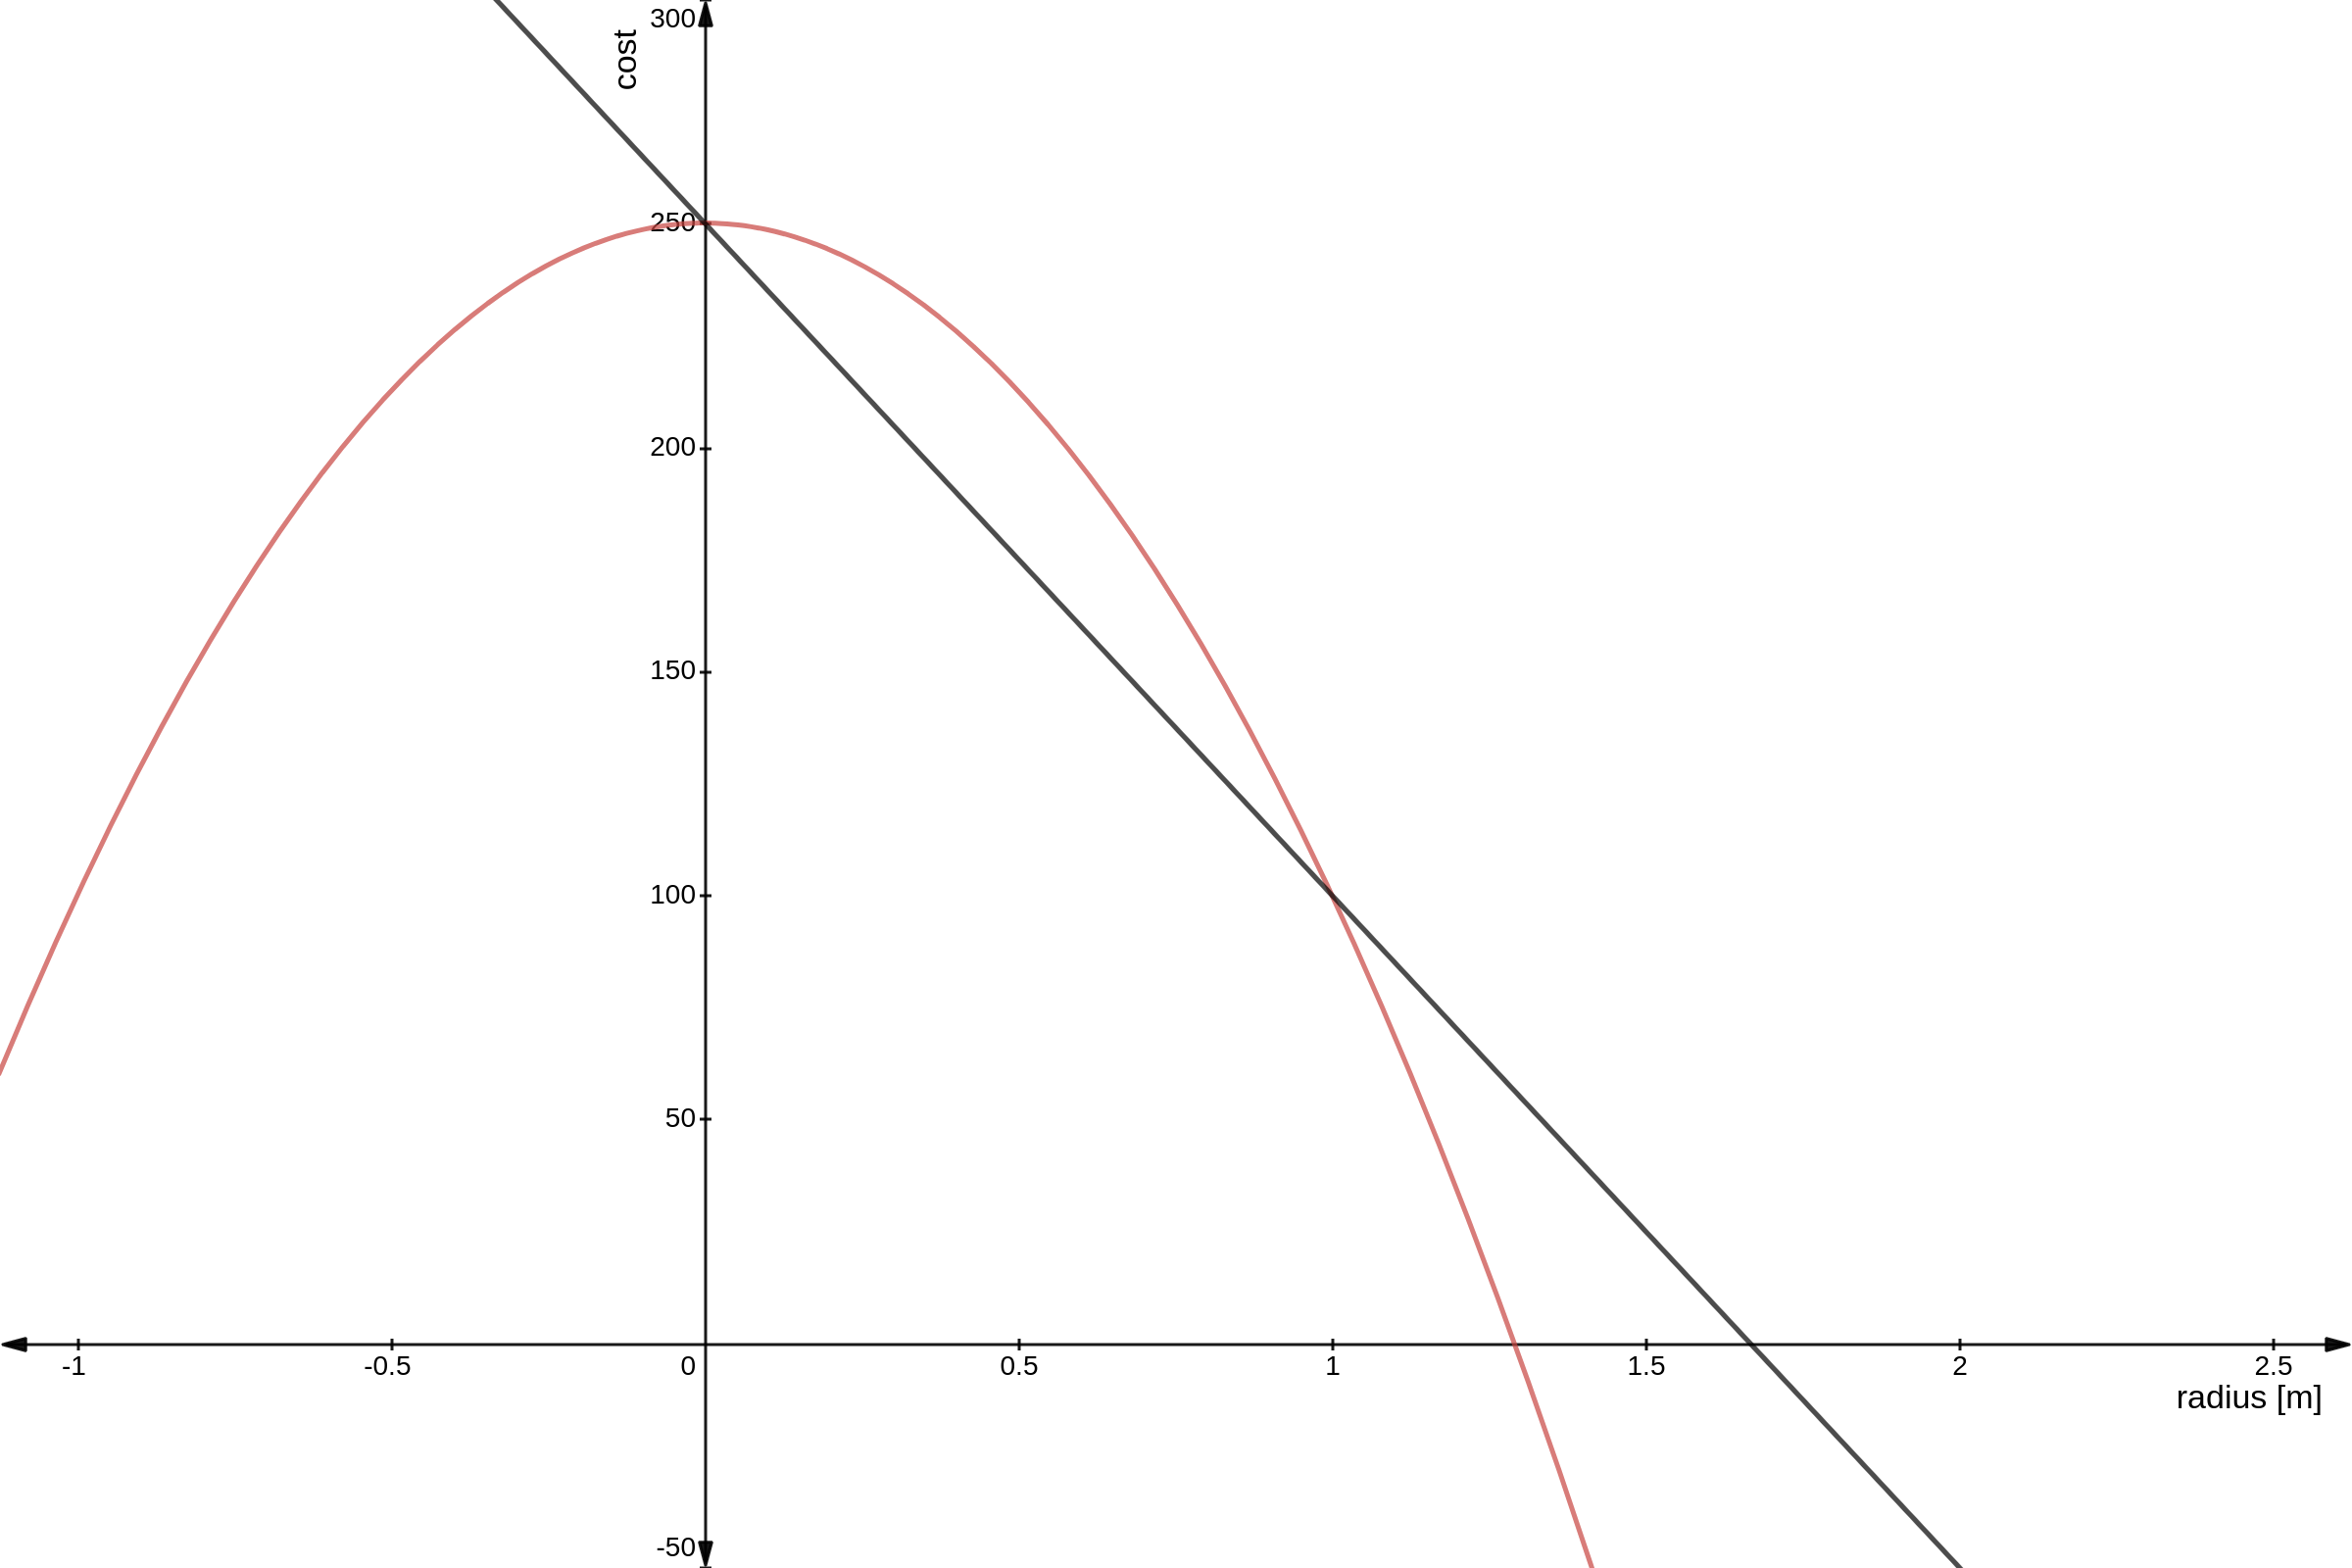
\includegraphics[width=140mm]{Pictures/linear cost comparison}
	\caption{cost distribution comparison with maxcost=250 mincost=100 radius=1}
	\end{center}
\end{figure}


\section{Planners}

\subsection{global\_planner}
There is not much room for configuration, when it comes to the global\_planner of the navigation\_stack. Probably the most important step for computation load is the choice of a planning algorithm.\\
The two algorithms that are offered by the global\_planner node are Dijkstra and A*.\\

Dijkstra does only consider the cost to the start node and determines the cost to get from the start node to every other node, until it finds the goal, from which it then can backtrack the shortest/cheapest path.\cite{AlgorithmenundDatenstrukturen}.\\

A* is based on the dijkstra algorithm but has one main difference. It considers not only the cost from the start to the current cell in the grid, but aswell a heuristic parameter, which is a general guess for the cost from the cell to the finish. The heuristic parameter is mostly bound to the euclidean distance between the cell in the grid and the finish. Like this the parameter will never over estimate the actual cost of the path\cite{AlgorithmenundDatenstrukturen}.\\

\begin{figure}[H]
	\begin{subfigure}{.5\linewidth}
		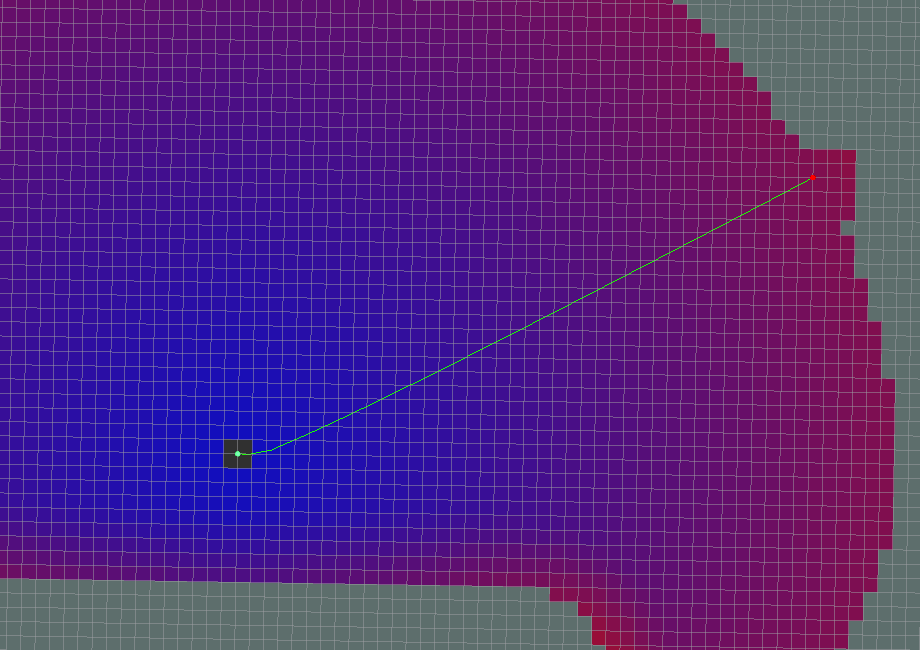
\includegraphics[width=\textwidth]{Pictures/Dijkstra}
		\caption{Dijkstra}
	\end{subfigure}	
	%\hskip2em
	\begin{subfigure}{.5\linewidth}
		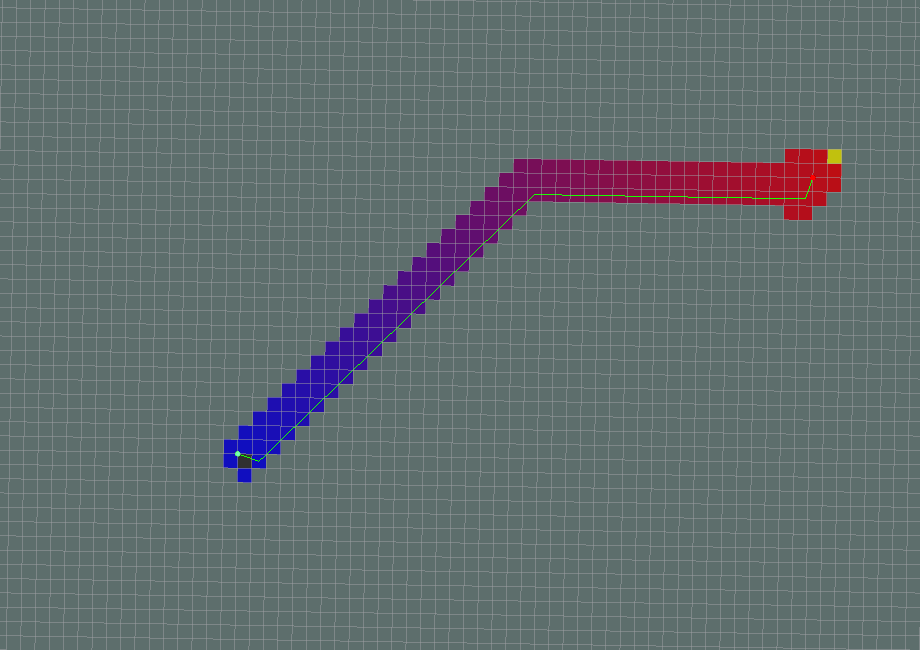
\includegraphics[width=\textwidth]{Pictures/AStar2}
		\caption{A*}
	\end{subfigure}

	\caption{planning algorithm comparison (grey cells are not observed)\cite{globalplanner}}
	\label{plannercomparison}

\end{figure}


It is obvious, that A* is much more efficient in this use case since the robot will mostly go straight or in a slight curve. Therefore A* will be chosen for the global planner.\\

Another important setting is necessary since the global costmap is used as a rolling window costmap. The global\_planner will be default outline the global costmap with lethal cost to prevent the global planner to plan outside of a fixed costmap. This behaviour results in artifacts, after the map has moved together with the robot which hinder the planners from finding a path.

\begin{figure}[H]
	\centering
	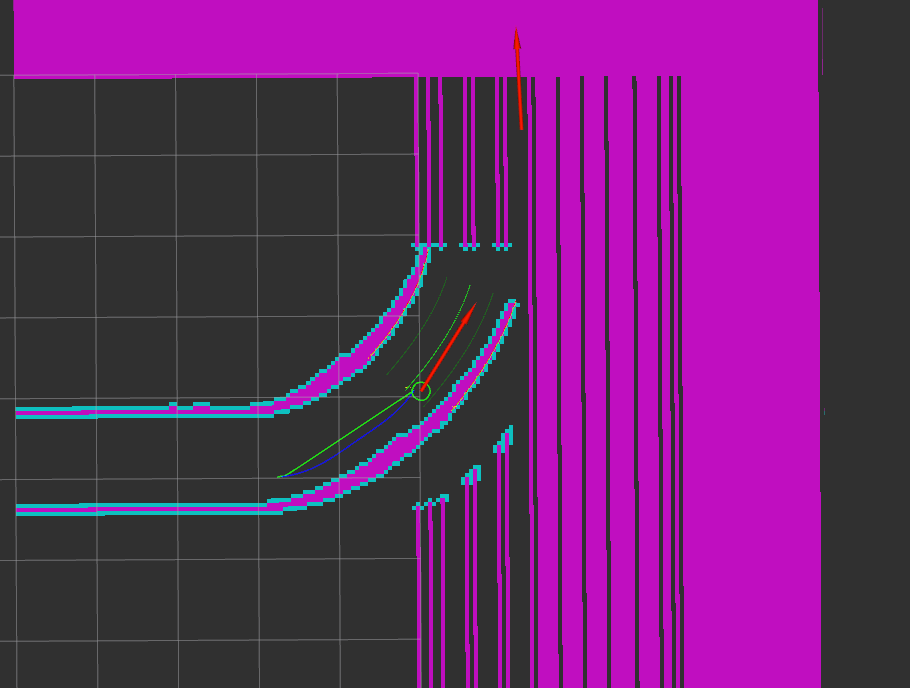
\includegraphics[width=\textwidth]{Pictures/borders}
	\label{boardererror}
	\caption{global planner border error}
\end{figure}

To prevent this behavior the not documented parameter ``outline\_map'' has to be set to false. The default value of this parameter is therefore changed in the forked version of the navigation stack.

To make planning easier the parameter ``cost\_factor'' can be reduced. This parameter multiplies the cost of every cell in the costmap before planning which
 would make the gradually decreasing cost of the dynamic\_cost\_layer redundant.

\subsection{teb\_local\_planner}

Like the global planner the local planner has to be configured to comply to the tasks the local planner has.

A good starting point for the configuration are the example configurations in the repository of the developer of the planner\cite{tebtutorials}. They offer base configurations for both differntial drive and car like, aswell as omnidirectional robots.\\

Unfortunately teb\_local\_planner only considers lethal cost and without any configuration would follow the global path very loosely resulting in e.g. cutting corners.\\ 

To give the planner a tendency to follow the global planner closer the option ``viapoint'' can be used. This allows to set points at a configurable distance to each other on the global path, that attract the local path and therefore pull the local path and the robot to the correct lane. The attraction of the local path through the via points is then tuned so the robot drives roughly in the middle of the right lane, when no obstacle is on the road, but still can separate itself from the global path, when avoiding obstacles.\\

The parameter ``max\_global\_plan\_lookahead\_dist'' controls how much of the global plan is actually considered by the local planner. This parameter highly influences the computational load when setting the distance to larger values. Using shorted distances results in oscillations while driving straight, which is caused by the jumping global path.






















